%
% Paper to be submitted to the Second International Conference
% on Advances in System Testing and Validation Lifecycle
% (VALID 2010), August 22--27, 2010 in Nice, France.
%
% For information on this file please contact Joe Loughry at
% Tel. +1 303 221 4380 (time zone GMT minus 7 hours) or Email:
% joe.loughry@stx.ox.ac.uk
%

\documentclass[10pt,letterpaper,conference,compsocconf]{IEEEtran}

\usepackage{cite}
\usepackage[english,british]{babel}
\usepackage[pdftex]{graphicx}

\usepackage[cmex10]{amsmath}
\interdisplaylinepenalty=2500

\usepackage{array}
% Frank Mittelbach's and David Carlisle's array.sty patches and improves
% the standard LaTeX2e array and tabular environments to provide better
% appearance and additional user controls. As the default LaTeX2e table
% generation code is lacking to the point of almost being broken with
% respect to the quality of the end results, all users are strongly
% advised to use an enhanced (at the very least that provided by array.sty)
% set of table tools. array.sty is already installed on most systems. The
% latest version and documentation can be obtained at:
% http://www.ctan.org/tex-archive/macros/latex/required/tools/

\usepackage{caption}
\usepackage[caption=false,font=footnotesize]{subfig}

\usepackage{fixltx2e}

\usepackage{url}

% *** Do not adjust lengths that control margins, column widths, etc. ***
% *** Do not use packages that alter fonts (such as pslatex).         ***
% There should be no need to do such things with IEEEtran.cls V1.6 and later.
% (Unless specifically asked to do so by the journal or conference you plan
% to submit to, of course. )

% correct bad hyphenation here
\hyphenation{op-tical net-works semi-conduc-tor}

\begin{document}

\title{Unsteady Ground: Certification to Unstable Criteria}

\author{
	\IEEEauthorblockN{Joe Loughry}
	\IEEEauthorblockA{Computing Laboratory \\
		University of Oxford \\
		Oxford, UK \\
		Email: joe.loughry@stx.ox.ac.uk
	}
}

\maketitle

\begin{abstract}
Cross Domain Systems for handling classified information
complicate the certification test and evaluation
problem, because along with multiple data owners comes duplicate
responsibility for residual risk.  Over-reliance on independent
verification and validation by certifiers and
accreditors representing different government agencies is interpreted as
conflating the principle of defence-in-depth with the practice of
repeated verification and validation testing.   Using real-world
examples of successful and unsuccessful certification test and
evaluation efforts to guide the development
of a new communication tool for accreditors, this research
aims to reduce time and cost wasted on unnecessary retesting of
the same or similar security requirements during
security test and evaluation in multi-level environments.
\end{abstract}

\def\IEEEkeywordsname{Keywords}

\begin{IEEEkeywords}
	cross domain systems; certification and accreditation;
	security test and evaluation; certification test and evaluation;
\end{IEEEkeywords}

\IEEEpeerreviewmaketitle

\section{Introduction}

What happens when a system that has been developed successfully under
one particular set of security testing criteria suddenly finds itself
needing to conform to a completely new set of rules?  The question is not
hypothetical; the same situation arises whenever a new certification scheme
is adopted, {\it e.g.}, the Common Criteria (CC) throughout its various revisions,
Health Insurance Portability and Accountability Act (HIPAA) and
Sarbanes--Oxley laws in the United States, or as regularly as clockwork
in the case of the peculiar species known as a Cross Domain System (CDS).
This paper aims to show that a lack of communication amongst government certifying
and accrediting agencies
leads to unnecessary duplication of effort and multiplication of cost with
no concomitant improvement in security.

The first part of this paper defines the term CDS and assurance
requirements for security accreditation.  Section~\ref{the-problem} describes
a particular security test and evaluation problem that is unique to CDS.
Section~\ref{examples} contains two real-world examples illustrating the
occurrence of the problem in practice.  Finally, Section~\ref{solution}
describes progress towards a solution.

\subsection{Characteristics of Cross Domain Systems}

CDSs handle classified information.  These systems are unlike other
installations that process classified information in that they encounter new or
changed security testing criteria all the time.
Unlike safety-critical systems, whose certification criteria are stable,
usually having been established by professional engineering organisations before
being given the weight of law~\cite{Leveson1994,Leveson1995,DO-178B,FAA8110.49-2003},
the security certification criteria under which classified data processing
systems are evaluated are ever-changing.
By definition, CDS installations always span at least one boundary between
security domains controlled by different data owners.  Data owners
do not trust one another with access to their data, hence the
need for a controlled interface between security enclaves~\cite{DCID-6/3a}.
An elementary
example of a CDS application is the one-way interface (sometimes called a
{\it data diode}) allowing wire
service news articles to flow into a classified intelligence-gathering
system (Figure~\ref{figure:simple-CDS}).
The purpose of a CDS is separation of security domains.  The
data owner of a classified system worries about two
potential threats: accidental leakage of classified information to
the unclassified side, called a {\it spill}, and the potential for
introducing malicious
code into the classified system from an outside source.

%
% Remove the "CLASSIFICATION MARKINGS ARE FOR ILLUSTRATIVE
% PURPOSES ONLY..." label on the bottom of the figure by
% adjusting the bottom trim value.  That way I can leave it
% in the figure file in case it's needed later.
%

\begin{figure}[!t]
    \centering
	% 'trim' specifies how much to remove from left, bottom,
	% right, and top edges of an A4 size PDF page.
	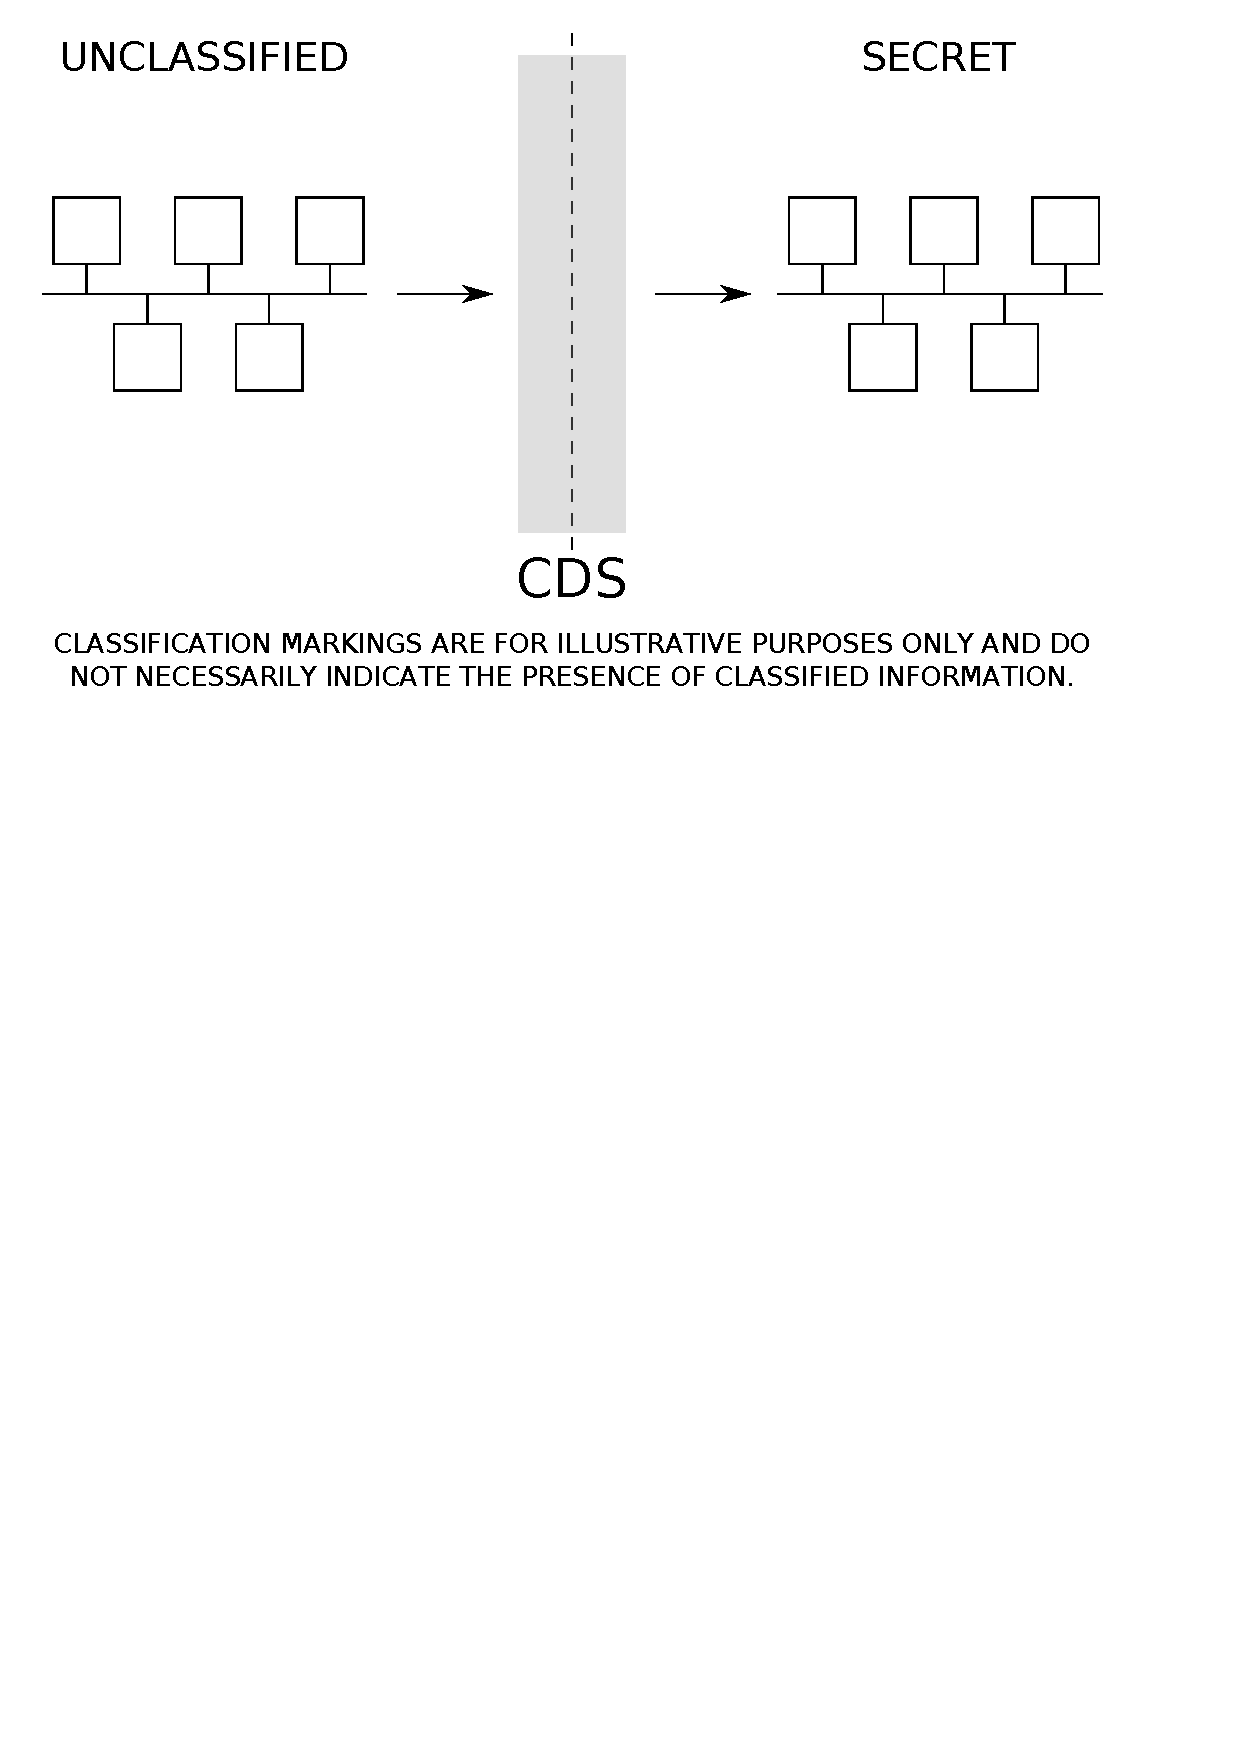
\includegraphics[width=0.5\textwidth,trim=0 19.25cm 2cm 0,clip]{simple-CDS.pdf}
	\caption{The simplest imaginable cross-domain system.}
	\label{figure:simple-CDS}
\end{figure}

The example shown in Figure~\ref{figure:simple-CDS} is simplistic because it
presupposes a unidirectional
flow of information from low to high (unclassified to classified) and
only two security domains.
More realistic CDS installations cope with bidirectional
flows---such as a web browser inside the security enclave that needs
to be able to search unclassified databases outside.  In practice,
multi-directional information flow requirements are commonplace.
Depending on the capability of the CDS, one system might handle scores
of channels simultaneously, interconnecting many security
domains at widely different classification levels.  Internally, the CDS
maintains separation of information by classification and source, routing
inputs to outputs according to rule sets specified by the data owners.
Advanced CDS systems have the capability to transform data in flight,
whether by transliterating message formats or by sanitising classified
information for release at a lower security level (Figure~\ref{figure:complex-CDS}).

%
% Again, take out the "CLASSIFICATION MARKINGS ARE..." obnoxious
% label on the bottom of the figure by adjusting the bottom trim
% value.
%

\begin{figure}[htbp]
    \centering
	% 'trim' specifies how much to remove from left,
	% bottom, right, and top edges of an A4 size PDF page.
	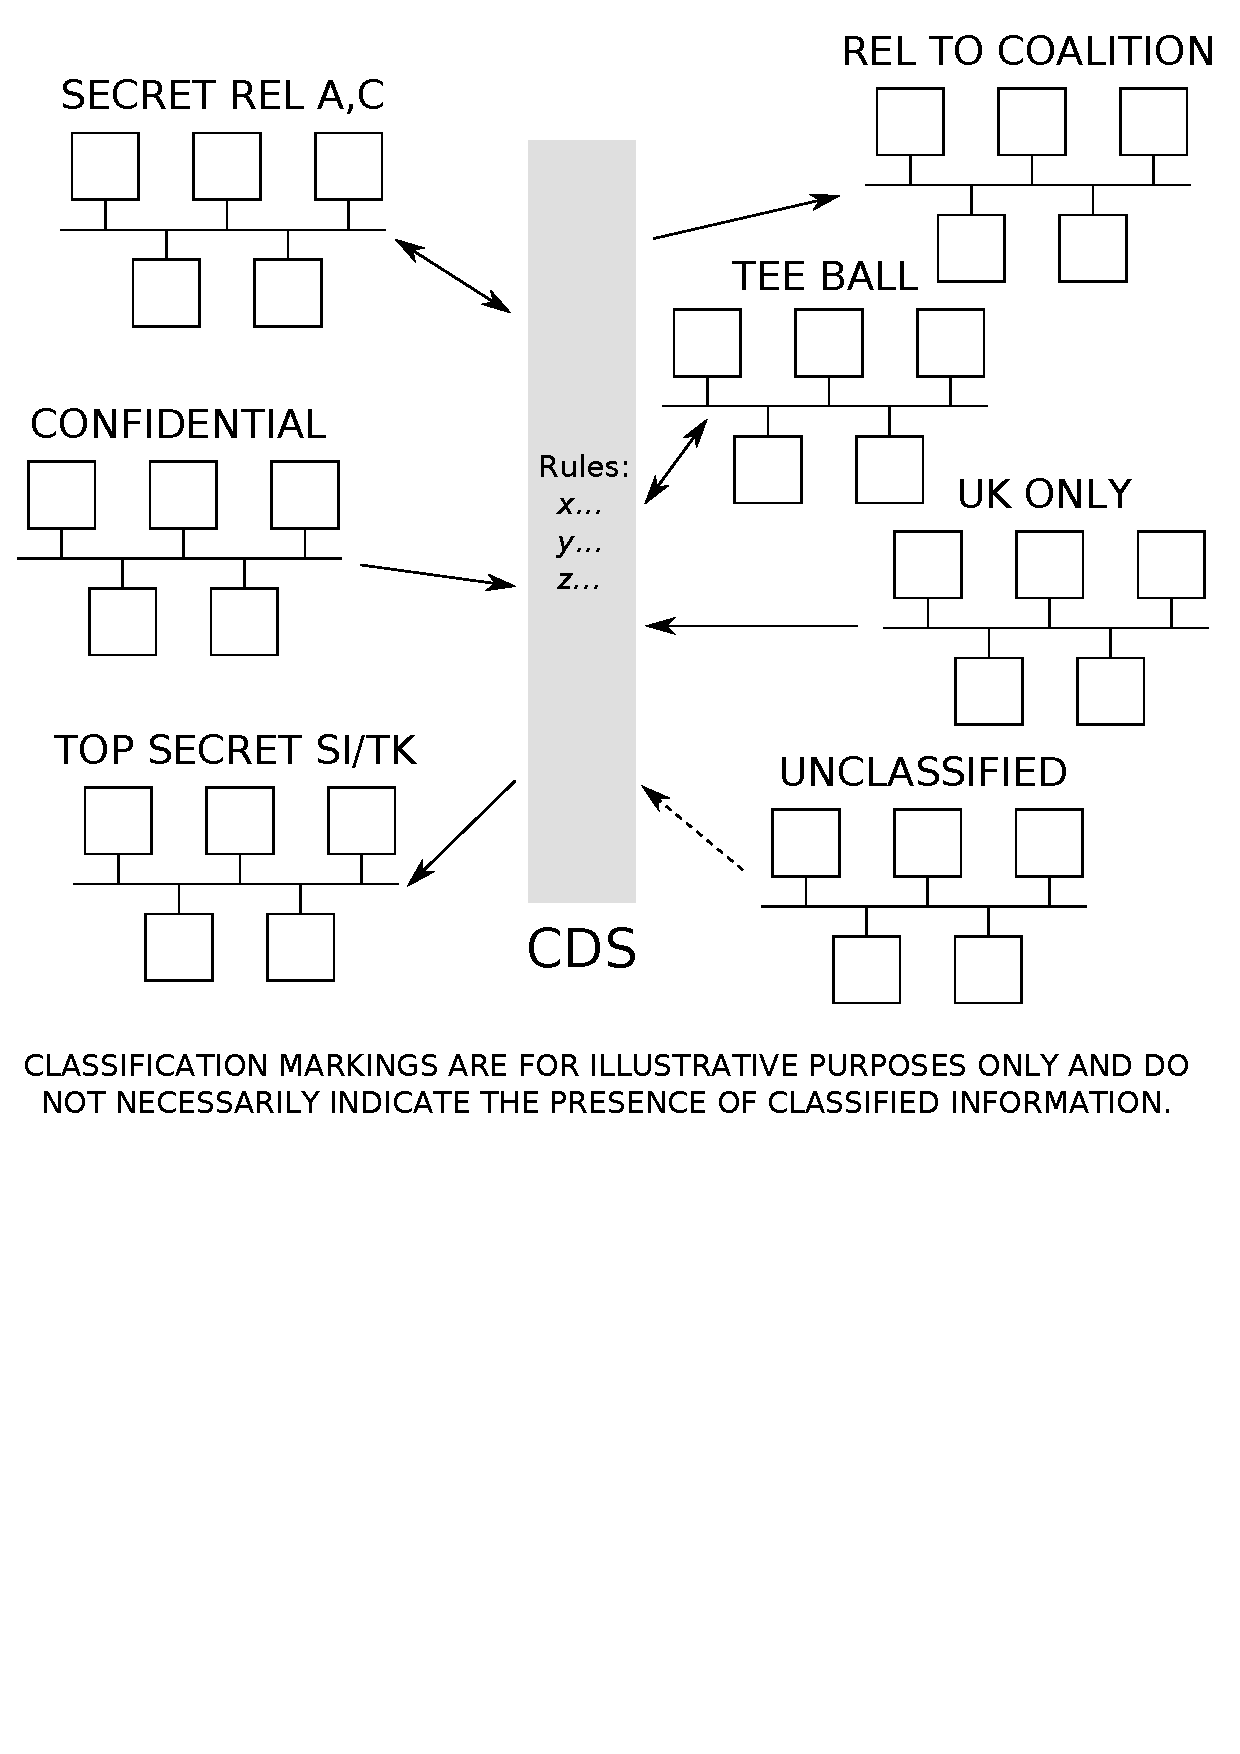
\includegraphics[width=0.5\textwidth,trim=0 12.25cm 0 0,clip]{complex-CDS.pdf}
	\caption{A more realistic CDS scenario with complex rules.}
	\label{figure:complex-CDS}
\end{figure}

\subsection{How Risk Reduction is Done and Measured}

As an irreducible result of inherent complexity, CDS
applications present a uniquely high
risk of failure whilst at the same time having the potential to cause
a great deal of damage to national security.  Consequently, they are
developed and tested with utmost care.  It begins with formalised
requirement and specification reviews, proceeding through software
development accompanied by systems and security engineering,
vetting of programme personnel, design and code inspections,
automated static analysis of source code, unit and system level
testing, configuration management of software and hardware, documentation,
training of installers and operators, audits, physical security, and
process improvement\cite{Anderson2008a,Fagan1976}.

Once software development is complete, the Certification Test
and Evaluation (CT\&E) phase
begins.
In the case of CDS applications having field-alterable rules,
CT\&E is performed using a representative set of processing rules
designed to exercise the capabilities of the system.
In practice, the software developer (being the one most familiar with the system)
creates an initial set of tests and expected results based on Factory
Acceptance Test (FAT) procedures and test coverage analysis.  Then a
different organisation is engaged to use
those procedures to perform Independent Verification and Validation
(IV\&V) and penetration testing on the system.  At each stage in the
certification process,
{\it findings}---deviations from expected results---are reported to the
developer and the certifier (Table~\ref{table:findings}).

After CT\&E, each instance of the CDS needs to be installed and accredited for
a particular use in a particular location.  After the initial site
survey, trained installers configure rule sets in coordination with
all of the data owners involved and set up the system in the location where
it is to be used, though it is not connected to all of the network endpoints yet.
At this time, site operations personnel, system administrators,
and security officers are trained on the new system.  Before the
CDS is allowed to connect for the first time, it needs to be tested one
more time in a process known as Security Test and Evaluation (ST\&E)
for accreditation.
Since the ultimate purpose of a CDS is to reduce residual risk to a
level acceptable by the data owner(s), in each case there is a Designated Approving Authority
(DAA)---a person delegated by the Principal Approving Authority (PAA)
of the data owner formally to accept responsibility for residual
risk in the operation of the CDS.  IV\&V contractors assist the DAA with
ST\&E by exercising the CDS through test procedures specific to the site
until the DAA is
satisfied and agrees to accept responsibility for the residual risk.
The DAA then issues an Approval to Connect (ATC) and allows the system
to operate.  The formal Approval to Operate (ATO) is for a limited
time---no more than three years---and contingent on security-relevant
changes not being made to the system without approval.

\begin{table}[!t]
	%% increase table row spacing, adjust to taste
	\renewcommand{\arraystretch}{2.0}

	% if using array.sty, it might be a good idea to tweak the value of
	% \extrarowheight as needed to properly center the text within the cells

	\caption{Categorisation of findings according to severity.}
	\label{table:findings}
	\centering
	\begin{tabular}{|c|l|}
		\hline
		% this uses a trick for centering table headings (required for IEEE style)
		{\bf Category} & \multicolumn{1}{c|}{\bf Relative Severity} \\ 
		\hline
		I & These are show-stoppers. \\
		\hline
		II & %
			\begin{minipage}{0.35\textwidth}
				\vspace{1mm}Less severe than a Cat I finding but must be
				corrected before CT\&E can proceed to completion\vspace{1mm}
			\end{minipage} \\
		\hline
		III & %
			\begin{minipage}{0.35\textwidth}
				\vspace{1mm}Do not necessarily prevent certification; fix may
				be deferred up to 180 days after Interim Approval
				to Operate (IATO)\vspace{1mm}
			\end{minipage} \\
		\hline
		IV & Minor problems, sometimes deferred indefinitely \\
		\hline
	\end{tabular}
\end{table}

The purpose of these four phases---trusted software development,
CT\&E, trusted delivery, and ST\&E---in combination is to reduce
the amount of risk to a level acceptable by the data owner.
The goal of the DAA is always to minimise residual risk.

%
% I decided that this figure is dumb.
%

% \begin{figure}[!t]
%     \centering
%	% 'trim' specifies how much to remove from left, bottom, right, and top of PDF page.
% 	\includegraphics[width=0.3\textwidth,trim=0 12cm 3cm 0,clip]{risk-and-weaknesses.pdf}
% 	\caption{Some bugs introduce no weakness (region $\alpha$), {\it e.g.}, misspelt words
% 		in a GUI; some exploitable weaknesses are not attributable to
% 		a bug (region $\beta$).  Residual risk (region $\gamma$) almost always includes known
% 		bugs that are not cost-effective to remove, or exploits
% 		that can never be completely prevented because they are inherent
% 		to the system, {\it e.g.}, denial-of-service.}
% 	\label{figure:residual-risk}
% \end{figure}

\section{The Problem}\label{the-problem}

All of the aforementioned steps are necessary to guarantee the level
of assurance needed by a CDS.  But it is at this point we argue that
the process loses coherence.  It was earlier mentioned that data owners
typically do not trust other data owners, at least not completely.  With
multiple data owners come multiple DAAs.  With multiple DAAs come repeated
rounds of ST\&E, typically conducted by the same IV\&V contractors---who,
being already familiar with the system, are the logical ones to test it
at a reasonable cost---and using similar or identical test procedures.

\begin{figure*}[!t]
    \centerline{
		\subfloat{
			% 'trim' specifies how much to remove from left, bottom, right, and top of PDF page.
			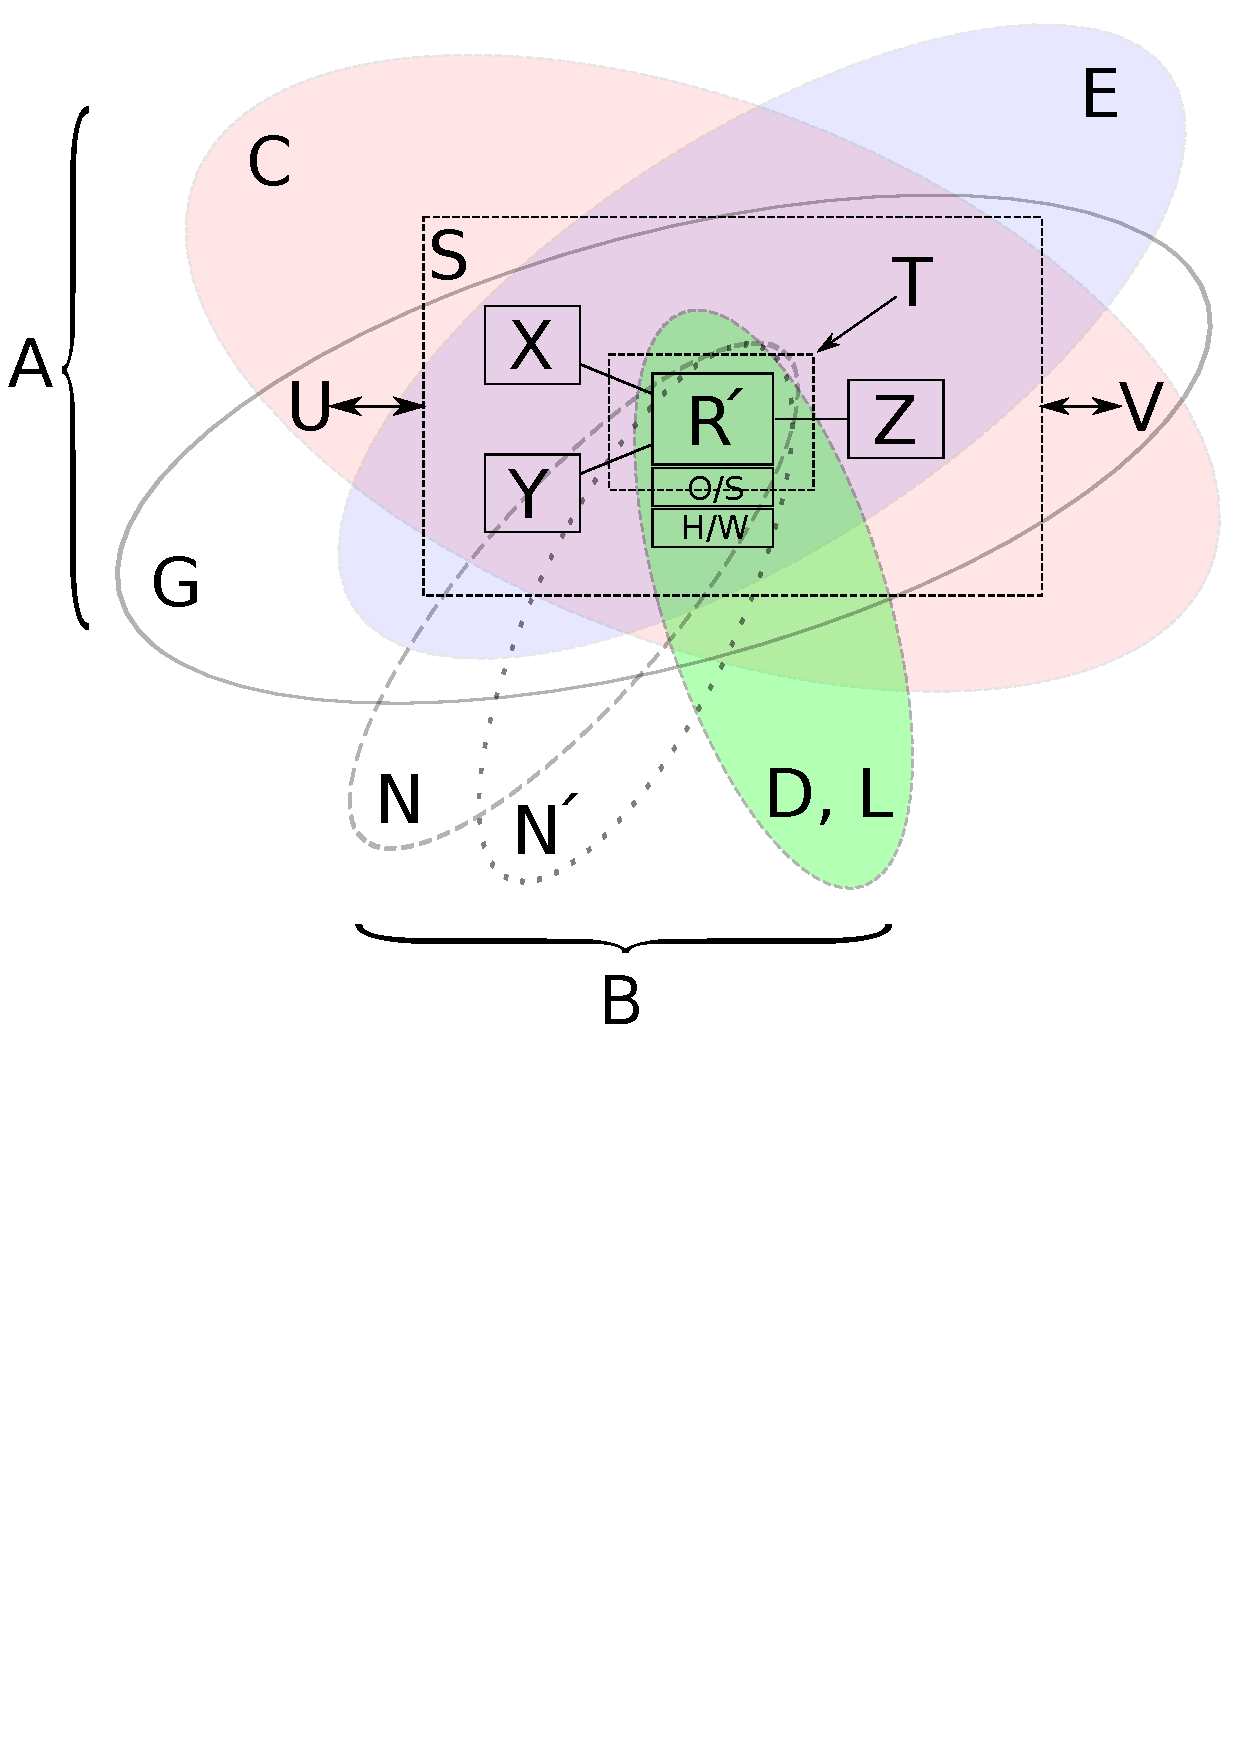
\includegraphics[width=0.45\textwidth,trim=0 11.5cm 0 0,clip]{R-prime-context-plus-N-prime.pdf}
			\label{figure:subfigure-a}
		}
		\hfill
		\subfloat{
			\begin{tabular}[b]{lp{5cm}}
				$A$ & Participants in country $A$ \\
				$B$ & Participants in country $B$ \\
				$C$ & Customer \\
				$D$ & Software developer \\
				$E$ & Systems integrator \\
				% $F$ & ? \\
				$G$ & $A$'s government security agency \\
				% $H$ & ? \\
				% $I$ & ? \\
				% $J$ & ? \\
				% $K$ & ? \\
				$L$ & CC testing Laboratory \\
				% $M$ & ? \\
				$N$ & $B$'s government security agency %
					for Common Criteria (CC) \\
				$N^\prime$ & Another government information-security %
					certifying agency of $B$ \\
				% $O$ & ? \\
				% $P$ & ? \\
				% $Q$ & ? \\
				% $R$ & $D$'s original product \\
				$R^\prime$ & The product being CC evaluated \\
				$S$ & System being developed by $E$ \\
				$T$ & TOE boundary \\
				$U$, $V$ & Other systems outside $S$ \\
				% $W$ & ? \\
				$X$, $Y$, $Z$ & Sub-components of $S$ \\
			\end{tabular}
			\label{figure:subfigure-b}
		}
	}
    \caption{Software developer $D$ had influence only
        over the Target of Evaluation (TOE) $R^\prime$, whereas the
        system as a whole was built by $E$.  When the customer's
        government security representative
        $G$ did their analysis, they considered the superset of
        $S^\ast$ including the external interfaces to $U$ and $V$.}
    \label{figure:context-diagram}
\end{figure*}

But this repeated testing at the ST\&E phase to the same or
similar criteria by different
government agencies would seem to be conflating the principle of
defence-in-depth with the practice of IV\&V.  If testing is
done competently, {\it i.e.}, following well-defined test
procedures based on established principles of test
coverage analysis and test design,
then it seems obvious that repeating effectively
the same tests---often performed by the same people according to scripts
derived from a common source---does not lead to increased
assurance~\cite[Chapter 13]{Beizer1990}, \cite[Chapter 14]{Kletz1999}.
Why does this situation arise?  It seems to be a
structural problem emergent from the compartmentalisation of esp.\ national
security systems.  To solve it, we can look at CT\&E as a testable
microcosm of ST\&E.

\section{Examples}\label{examples}

As evidence that the problem is real, consider the following
examples of the same CDS under different circumstances.

\subsection{An Unsuccessful Common Criteria Evaluation}

The Common Criteria for Information Technology Security Evaluation
is an ISO standard for developers to show that
products satisfy specified security requirements to a specified
level of assurance.

The original motivation for this research derived from events related
to a military communications software project in 2006.  The example
has been anonymised for national security reasons.  Customer $C$ in
country $A$ ordered
a complex system $S$ to be built (Figure~\ref{figure:context-diagram})
by systems integrator $E$.
One component of the system proposed by $E$ was to be $R^\prime$---a
slight variant of $R$, a mature and well-regarded
product of the $D$ corporation in country $B$.  $R$ had been
evaluated for security by $N^\prime$ (and other government agencies)
numerous times before.
Acting as a subcontractor to $E$ on the project, $D$ made the necessary
alterations to $R$.  (In reality, $D$ and $E$ were two branches of
the same company, not an uncommon occurrence in large organisations.)
The customer imposed an additional requirement, however:
$R^\prime$ needed to have a Common Criteria certificate, which
$R$ did not yet have.
$D$ felt that CC evaluation presented no great difficulty, as $R$
had endured many similar security certifications over the past decade;
satisfying the CC ought to be no great burden and as a bonus, $R$
would benefit from the---quite expensive---evaluation of $R^\prime$.
An authorised CC testing
laboratory, $L$ was engaged to assist with the security evaluation
of $R^\prime$.
$D$ and $L$ worked together to assemble the voluminous
documentation required to make their case before $N$, the CC certifier
in country $B$ that would formally evaluate the security of $R^\prime$.

Shortly before the evaluation documentation of $R^\prime$ was to be
delivered to $N$ for formal security
evaluation, $C$ made the overall system $S^\ast$ available to $G$, their
government's most trusted information security adviser.  $G$ pronounced
$S$ `not fit for purpose' and recommended against its adoption.
$C$ cancelled the
project, and soon after funding dried up, the CC evaluation of
$R^\prime$ was abandoned.

What can be learnt from this example?  The
software should not have failed its CC evaluation.  It had previously
withstood
numerous, rigorous, and repeated security evaluations over a period
of more than ten years.  In a sense, the root cause of the failure
was a requirements change,
but it was a change in the environment having nothing to do with
functionality.  Nevertheless, major shifts in CT\&E criteria are a
fact of life for CDS developers and the development methodology must
acknowledge this.

\subsection{DIACAP Certification}

The second example has to do with a U.S.\ Department of Defense
(DOD) Information Assurance Certification and Accreditation Programme
(DIACAP) certification of $R^{\prime\prime}$, a later version of
the original system $R$ from the first example.

Is there a difference in the post-CT\&E software defect rate,
measured in terms of the number of Category I--IV findings
between different versions of the same system in subsequent rounds
of ST\&E by different DAAs?  (See Figure~\ref{figure:thesis-question}.)
Data from approximately five rounds of CT\&E and penetration testing
conducted by $N^\prime$ and other agencies over a five-year period
on successive versions of $R$ and $R^{\prime\prime}$ are available.
The answer to the question in Figure~\ref{figure:thesis-question}
will give us a quantitative way of measuring the efficacy
of CT\&E methodology {\it vis-\`{a}-vis} CDS the way it is done
today.

\begin{figure}[!t]
    \centering
	% 'trim' specifies how much to remove from left, bottom,
	% right, and top of an A4 size PDF page.
	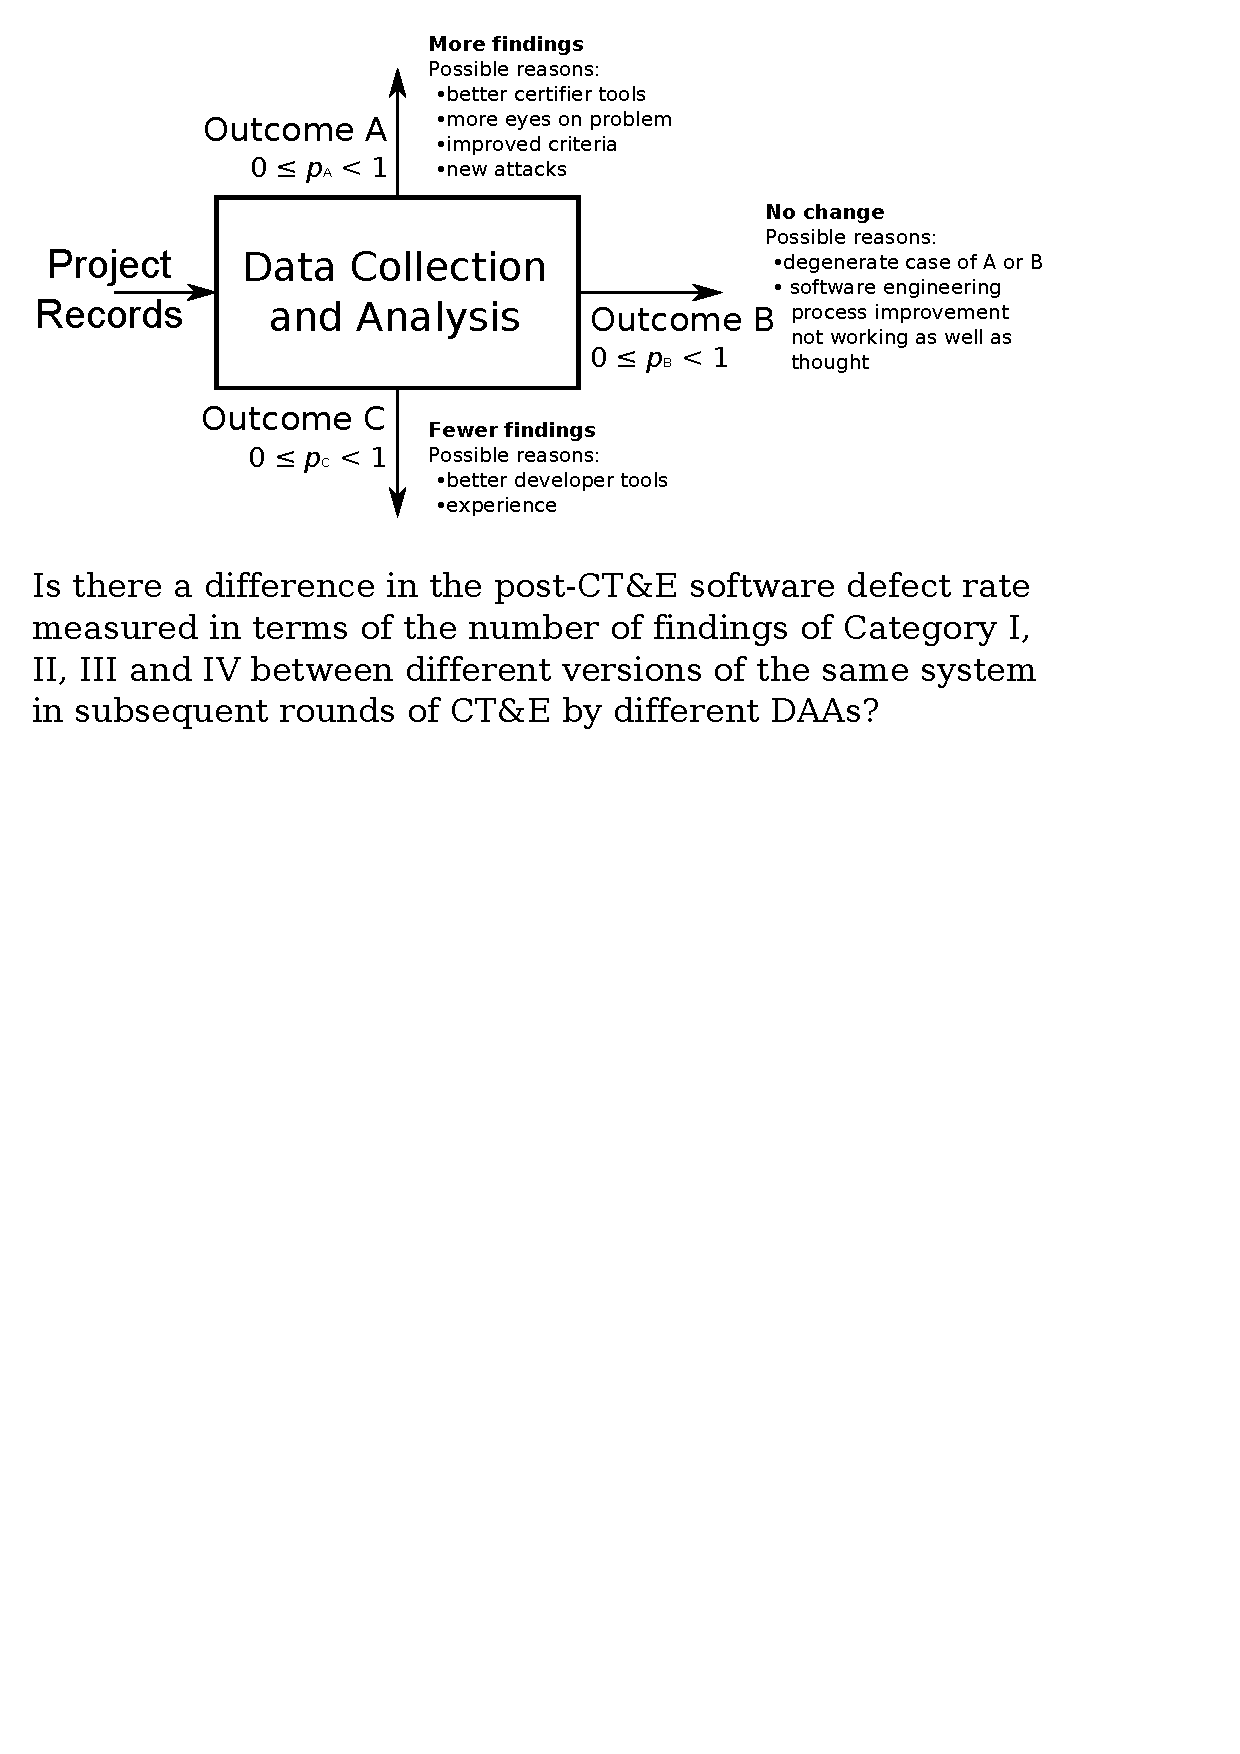
\includegraphics[width=0.5\textwidth,trim=0 20.5cm 3cm 0,clip]{thesis-question.pdf}
	\caption{Is there a difference in the post-CT\&E software
		defect rate between different versions of the same
		system in subsequent rounds of ST\&E by different
		DAAs?}
	\label{figure:thesis-question}
\end{figure}

This is a prime example of the most general case of certification to
unstable criteria: when a new standard replaces an older one and
developers of existing products are forced to switch over.
The software has outlived its evaluation criteria.  In the case
of $R^{\prime\prime}$,
Director of Central Intelligence Directive (DCID) 6/3 is being
replaced by the National
Institute of Standards and Technology (NIST) Special Publication
(SP) 800-53, which defines an entirely new set of security
controls along with the risk management framework in
NIST SP 800-37 under
DIACAP~\cite{DCID-6/3a,NIST-SP800-53r3,NIST-SP-800-53A2,NIST-SP-800-37,DIACAP}.
What is unique
about this example is that the certifiers are learning the new
standard at the same time as the developer---$R^{\prime\prime}$
is the first system
to undergo NIST SP 800-53 certification as it replaces DCID 6/3.
So far, certification is proceeding normally, without
any of the problems that occurred during the CC evaluation of
$R^\prime$.

Secondly, by observing the activity of developers, certifiers,
IV\&V, and DAAs throughout the process of CT\&E and ST\&E on a
new version of an existing CDS, it should be possible to elucidate
the ideal amount of inter-DAA communication consistent with a
minimum of duplicated testing to a defined level of security
assurance.

\section{Proposed Solution}\label{solution}

Security accreditation of CDSs ultimately comes down to a relatively
small number of people.  A new tool being developed at the University
of Oxford, called {\it nihil obstat}, is designed to facilitate concord
amongst DAAs by presenting test procedures and test results in a form acceptable
to all of the DAAs responsible for ST\&E accreditation of a particular
CDS.

The theory that informs the design of the tool characterises
residual risk as a function of multiple DAAs with a range of security
clearances who know about different sets of risk and risk
mitigations that are at least partly disjoint.
Each data owner perceives a set of risks $A_i$ that would be desirable
to mitigate, a set of risks $B_i$ it is possible to mitigate, and their
relative complement $R = A_i - B_i$, being the residual risk known to
that accreditor.  If we can prove to subsequent DAAs that the aggregate
residual risk is less than $R_i$, then repeated rounds of ST\&E may be
avoided.

% $R = \bigcup\limits_{i=1}^n R_i < R_i$

\section{Conclusion and Future Work}

Cross Domain Systems are unique because they exist in the
intersection
of stringent security requirements and ever-changing standards.  They
are different from safety-critical systems in two important ways:
firstly, safety-critical standards do not change as rapidly as security
standards do; and secondly, CDSs are {\it always} located on the
disputed borderlands between mutually distrusting security domains.
With multiple data owners come multiple responsible authorities (DAAs)
and with multiple DAAs come repeated rounds of the same or similar
tests, without any concomitant improvement in security assurance.  The
problem seems amenable to solution by a process of
gathering, collation, and presentation of test procedures and test
results to DAAs in a neutral format.  A pair of related examples yield
real-world experience with unstable criteria---both successful and
unsuccessful---derived from contiguous versions of a single CDS spanning
more than a decade.  CT\&E is more visible, but ST\&E happens all the
time and can be streamlined.

% Note that IEEE typically puts floats only at the top, even when this
% results in a large percentage of a column being occupied by floats.

% Note that IEEE does not put floats in the very first column - or typically
% anywhere on the first page for that matter. Also, in-text middle ("here")
% positioning is not used. Most IEEE journals/conferences use top floats
% exclusively. Note that, LaTeX2e, unlike IEEE journals/conferences, places
% footnotes above bottom floats. This can be corrected via the \fnbelowfloat
% command of the stfloats package.

\section*{Acknowledgement}

I would like to thank my supervisor, Andrew Martin
for his advice and encouragement; Joanna Ashbourn for teaching me
scientific writing; Cornelius Namiluko and John Lyle for their
insightful comments; Olav Kjono for access to data;
Steve Steinberger for conversations over coffee and help with interpretation;
and Chip Auten and Annie Cruz for mentoring.

% trigger a \newpage just before the given reference
% number - used to balance the columns on the last page
% adjust value as needed - may need to be readjusted if
% the document is modified later
%\IEEEtriggeratref{8}
% The "triggered" command can be changed if desired:
%\IEEEtriggercmd{\enlargethispage{-5in}}

\bibliographystyle{IEEEtran}
\bibliography{IEEEabrv,consolidated_bibtex_file}

\end{document}

